\documentclass[a4paper,12pt,french]{article}
\usepackage[margin=2cm]{geometry}
\usepackage[thinfonts]{uglix2}
\nouveaustyle
\pagestyle{empty}

\begin{document}
\titre{Réseaux et routage - Exercices 2}{NSI2}{2022} 

\begin{exercice}[ : Comparaison RIP/OSPF]
On 	considère le réseau suivant 
\begin{center}
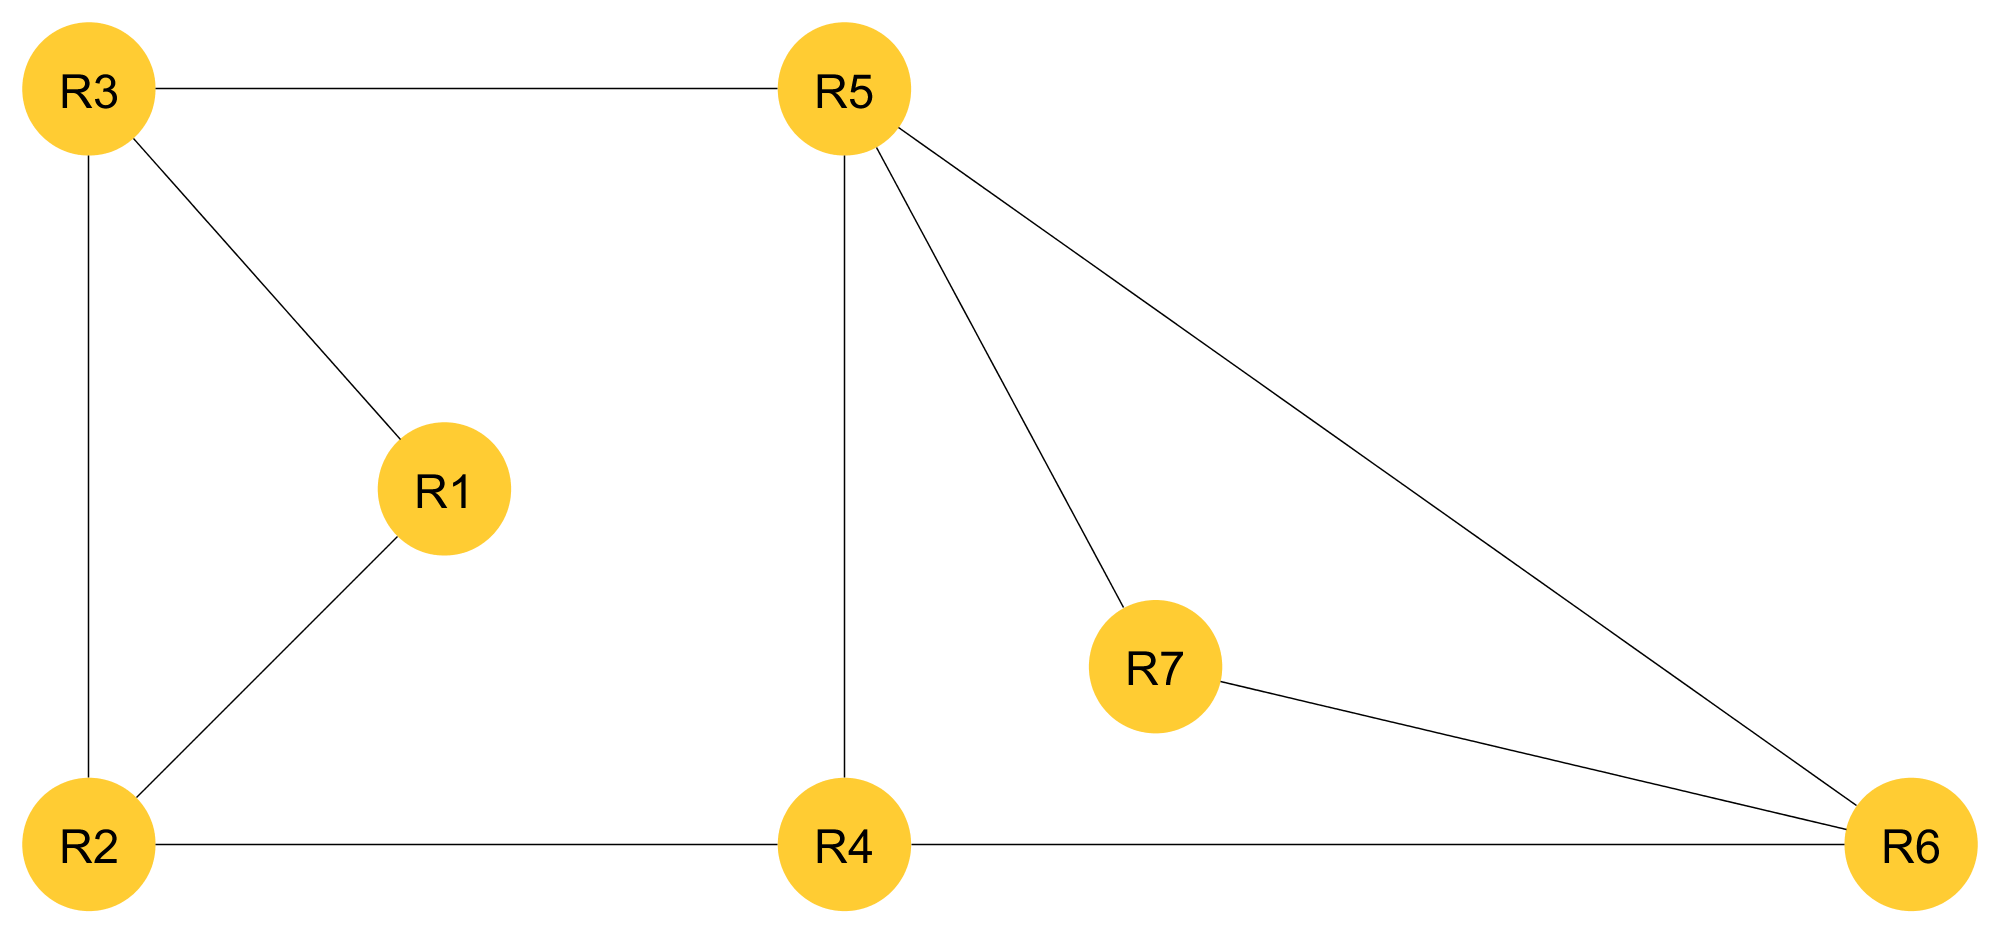
\includegraphics[width=14cm]{img/rip}
\end{center}

\textbf{1.} Si les routeurs suivent le protocole RIP, quel est la route empruntée par un paquet acheminé de R1 vers R7 ? Justifier.

\textbf{2.} Les routeurs sont maintenant configurés suivant le protocole OSPF. Les débits des interconnexions sont reportés ci-dessous :
\begin{center}
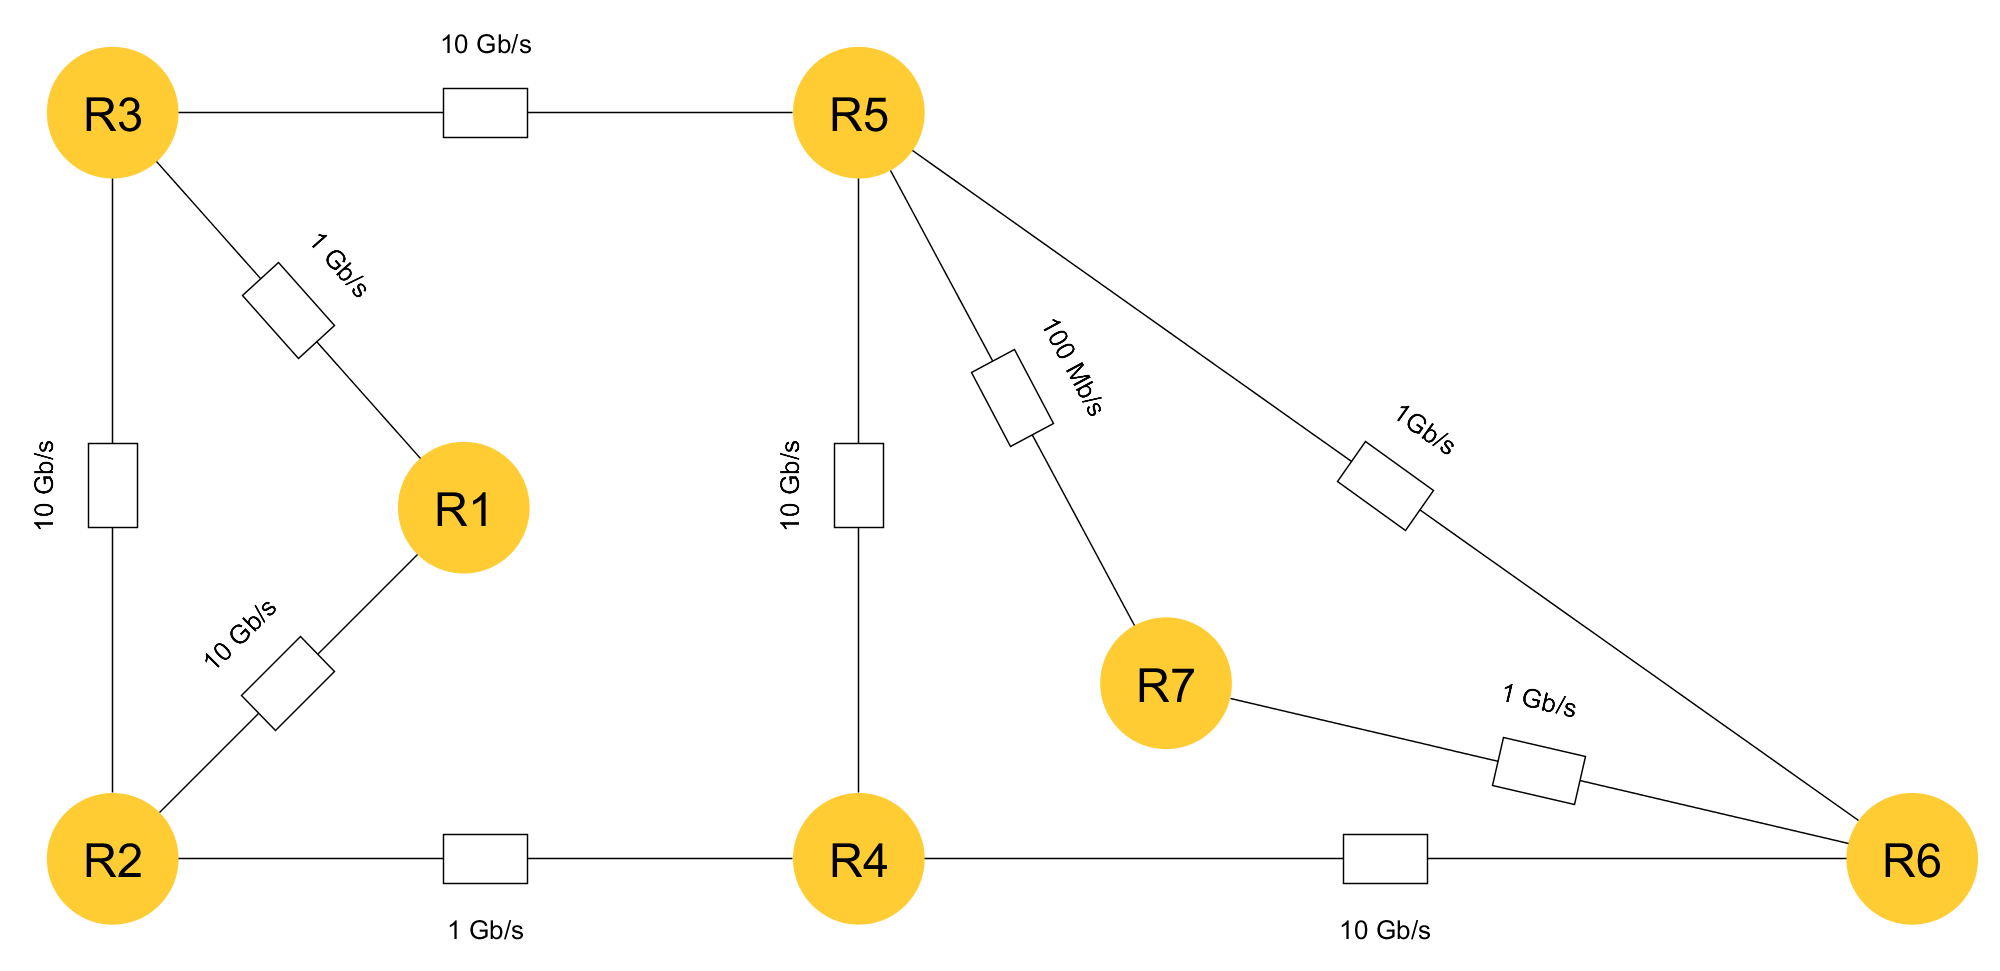
\includegraphics[width=14cm]{img/ospf}
\end{center}
\begin{enumerate}[\bfseries a.]
\item 	Reporter sur le graphe les coûts des connexions.
\item 	On veut connaître le chemin emprunté par un paquet transitant de R1 vers R7. Compléter le tableau ci-dessous en 
appliquant l'algorithme de Dijkstra et conclure.

\begin{center}
\begin{tabular}{|c|c|c|c|c|c|c|}
	\hline
	\rowcolor{orange}		\ \ \textbf{\color{white}R1}\ \  & \ \ \textbf{\color{white}R2}\ \ &\ \  \textbf{\color{white}R3}\ \  &\ \  \textbf{\color{white}R4}\ \  &\ \  \textbf{\color{white}R5}\ \  &\ \  \textbf{\color{white}R6}\ \  &\ \  \textbf{\color{white}R7}\ \  \\
	\hline
	\rowcolor{white}& & & & & & \\
	\rowcolor{white}& & & & & & \\
	\rowcolor{white}& & & & & & \\
	\rowcolor{white}& & & & & & \\
	\rowcolor{white}& & & & & & \\
	\rowcolor{white}& & & & & & \\
	\rowcolor{white}& & & & & & \\
	\rowcolor{white}& & & & & & \\
	\rowcolor{white}& & & & & & \\
	\rowcolor{white}& & & & & & \\
	\rowcolor{white}& & & & & & \\
	\rowcolor{white}& & & & & & \\
	\hline														\end{tabular}

\end{center}
\item Quel est le coût de la route choisie par le protocole RIP ?
\end{enumerate}
\end{exercice}
\end{document}